
\begin{figure*}[t!]
	\centering
	\begin{subfigure}[b]{0.33\textwidth}
		\centering
		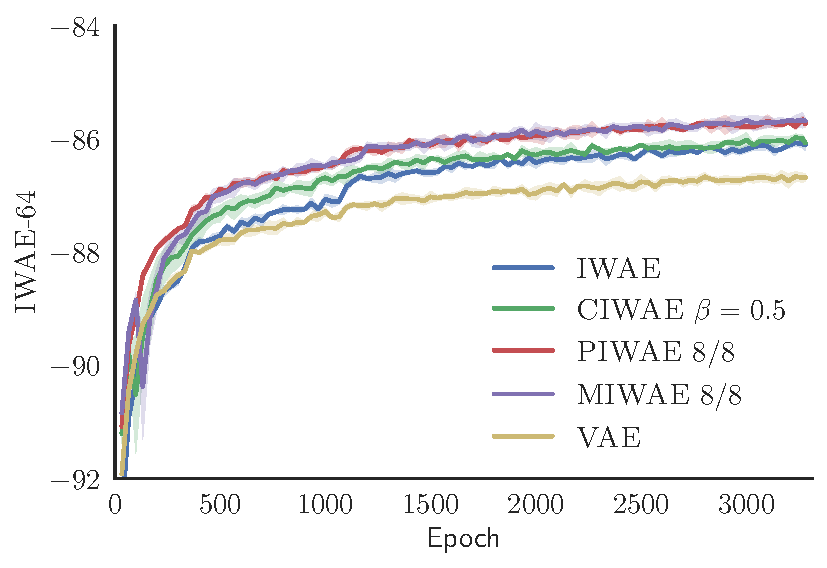
\includegraphics[width=\textwidth]{figures/tighter_bounds/convergence_IWAE_64}
		\caption{\textsc{IWAE}$_{64}$ \label{fig:mnistexpt/convergence/iwae64}}
	\end{subfigure}
	\begin{subfigure}[b]{0.33\textwidth}
		\centering
		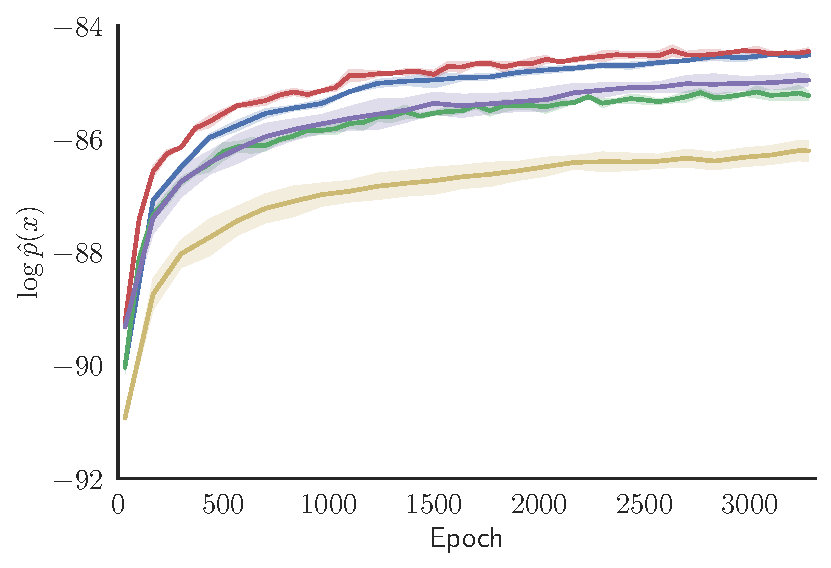
\includegraphics[width=\textwidth]{figures/tighter_bounds/convergence_log_p(x)}
		\caption{$\log \hat{p}(x)$ \label{fig:mnistexpt/convergence/logpx}}
	\end{subfigure}
	\begin{subfigure}[b]{0.33\textwidth}
		\centering
		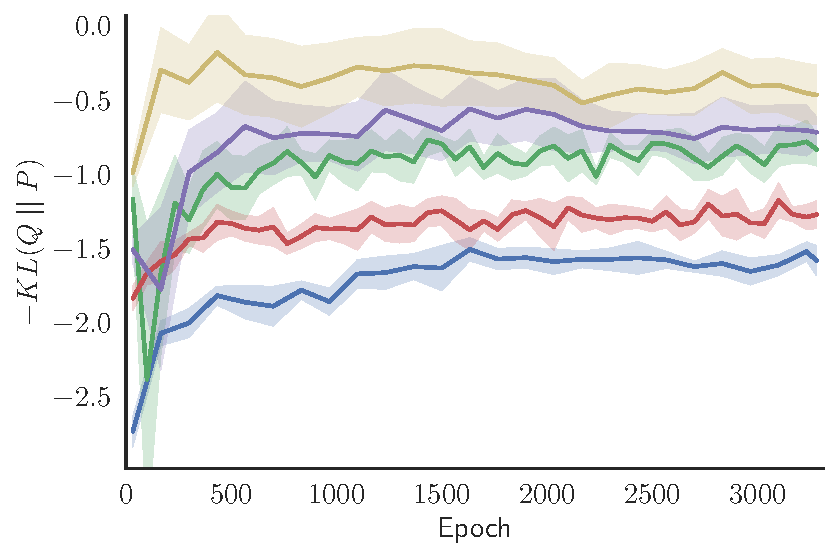
\includegraphics[width=\textwidth]{figures/tighter_bounds/convergence_KL}
		\caption{$-\mathrm{KL}(Q_{\phi}(z \given x) || P_{\theta}(z \given x))$ \label{fig:mnistexpt/convergence/kl}}
	\end{subfigure}\vspace{-6pt}
	\caption{Convergence of evaluation metrics on the test set with increased training time. 
		All lines show mean $\pm$ standard deviation 
		over 4 runs with different random
		initializations. Larger values are preferable for each plot.
		\vspace{-8pt}  \label{fig:mnistexpt/convergence}}
\end{figure*}

\begin{figure*}[t!]
	\centering
	\begin{subfigure}[b]{0.33\textwidth}
		\centering
		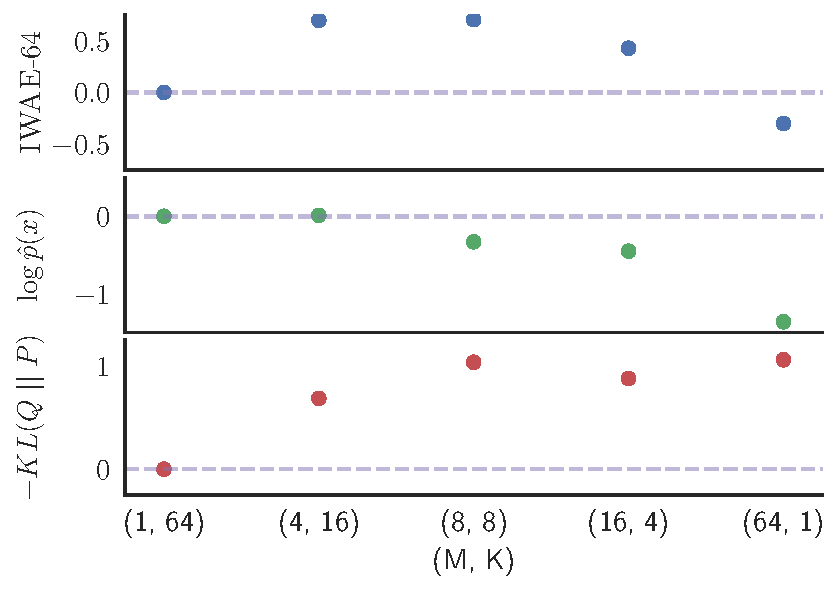
\includegraphics[width=\textwidth]{figures/tighter_bounds/combinations_miwae}\
		\caption{Comparing \gls{MIWAE} and \gls{IWAE} \label{fig:mnistexpt/dotplot/miwae}}
	\end{subfigure}
	\begin{subfigure}[b]{0.33\textwidth}
		\centering
		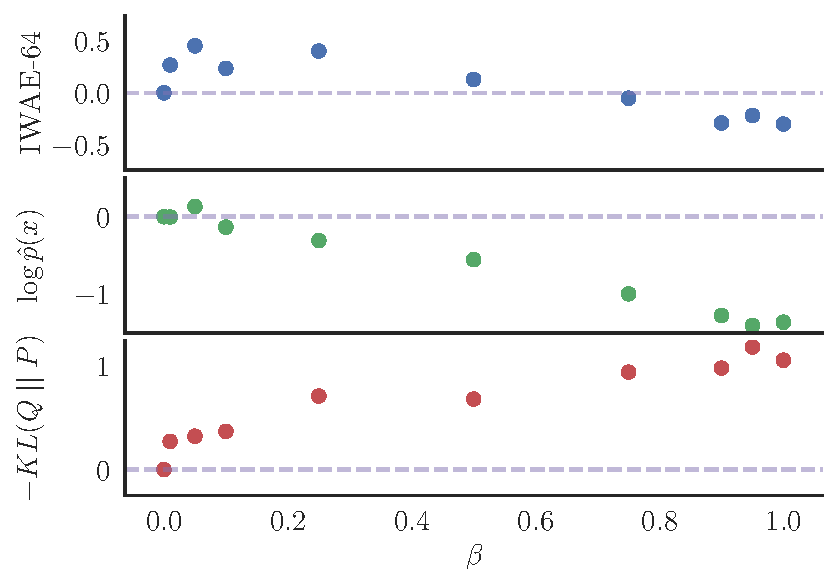
\includegraphics[width=\textwidth]{figures/tighter_bounds/combinations_combo}\
		\caption{Comparing \gls{CIWAE} and \gls{IWAE} \label{fig:mnistexpt/dotplot/ciwae}}
	\end{subfigure}
	\begin{subfigure}[b]{0.33\textwidth}
		\centering
		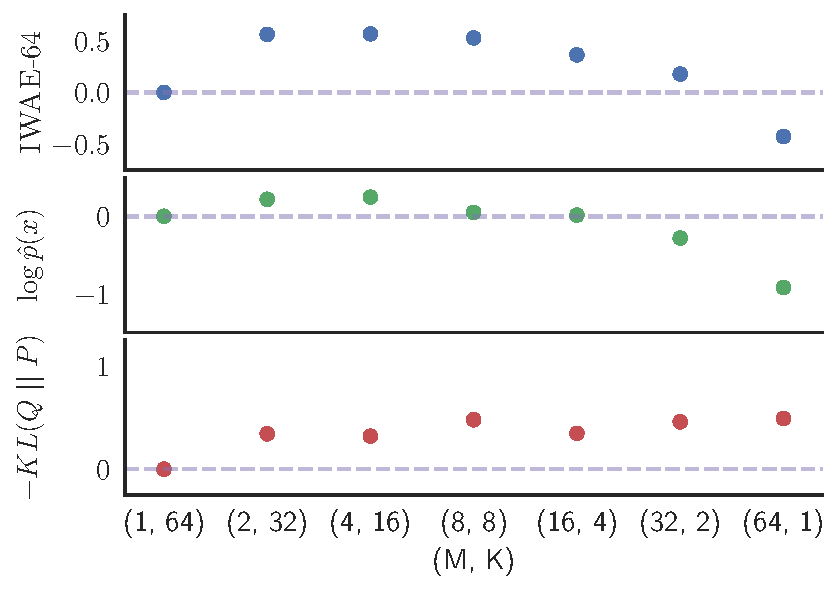
\includegraphics[width=\textwidth]{figures/tighter_bounds/combinations_piwae}
		\caption{Comparing \gls{PIWAE} and \gls{IWAE} \label{fig:mnistexpt/dotplot/piwae}}
	\end{subfigure} \vspace{-12pt}
	\caption{Test set performance of \gls{MIWAE}, \gls{CIWAE}, and \gls{PIWAE} relative to \gls{IWAE} in terms of the \gls{IWAE}-64 (top), $\log \hat p(x)$ (middle), and $-\mathrm{KL}(Q_{\phi}(z \given x) || P_{\theta}(z \given x))$ (bottom) metrics.  All dots are the difference in the metric to that of~\gls{IWAE}. Dotted line is the \gls{IWAE} baseline.
		Note that in all cases, the far left of the plot correspond to
		settings equivalent to the \gls{IWAE}.\vspace{-8pt} 	 \label{fig:mnistexpt/dotplot}}
\end{figure*}

\begin{table*}[t!]                        
	\centering    
	\scriptsize             
	\setlength\tabcolsep{2.5pt}	  
	\renewcommand{\arraystretch}{1.2}          
	\caption{Mean final test set performance $\pm$ standard deviation over $4$ runs. Numbers in brackets indicate $(M,K)$.
		The best result is shown in red, while bold results are not
		statistically significant to best result at the 5\% level of a Welch's t-test. \vspace{-8pt} \label{table:final-pef}}                    
	\begin{tabular}{|c|cccccccc|}                    
		\hline                                                       
		Metric & \gls{IWAE} & \gls{PIWAE} $(4,16)$ & \gls{PIWAE} $(8,8)$ & 
		\gls{MIWAE} $(4,16)$ & \gls{MIWAE} $(8,8)$ & \gls{CIWAE} $\beta=0.05$ & \gls{CIWAE} $\beta=0.5$ & \gls{VAE}     \\
		\hline    
		\gls{IWAE}-$64$ 
		& --$86.11\pm 0.10$ 
		& {\bf--}$\mathbf{85.68\pm 0.06}$ & {\bf--}$\mathbf{85.74\pm 0.07}$ 
		& {\color{red} \bf --$\mathbf{85.60\pm 0.07}$} & {\bf--}$\mathbf{85.69\pm 0.04}$ 
		& --$85.91\pm 0.11$ & --$86.08\pm 0.08$  
		& --$86.69\pm 0.08$ \\ 
		$\log \hat{p}(x)$ 
		& {\bf--}$\mathbf{84.52\pm 0.02}$  
		& {\color{red} \bf --$\mathbf{84.40\pm 0.17}$} 	& {\bf--}$\mathbf{84.46\pm 0.06}$ 
		& {\bf--}$\mathbf{84.56\pm 0.05}$ & --$84.97\pm 0.10$	 
		& 	{\bf--}$\mathbf{84.57\pm 0.09}$ & --$85.24\pm 0.08$  
		& --$86.21\pm 0.19$ \\ 
		$-\mathrm{KL}(Q|| P)$ 
		& --$1.59\pm 0.10$ 
		& --$1.27\pm 0.18$ & --$1.28\pm 0.09$ 
		& {\bf--}$\mathbf{1.04\pm 0.08}$ & {\bf--}$\mathbf{0.72\pm 0.11}$  
		& --$1.34\pm 0.14$ & {\bf--}$\mathbf{0.84\pm 0.11}$ 
		& {\color{red} \bf --$\mathbf{0.47\pm 0.20}$} \\ 
		\hline                                
	\end{tabular}                 
	\vspace{-12pt}                                           
\end{table*} 

\subsection{Experiments}
\label{sec:exp-algs}

We now use our new estimators to train deep generative models for the MNIST digits 
dataset~\citep{Lecun1998gradient}.  For this, we duplicated the 
architecture and
training schedule outlined in~\citet{Burda2016importance}. In particular, all networks were trained and evaluated using their
 stochastic binarization.
For all methods we set a budget of $T=64$ weights in the target estimate
for each datapoint in the minibatch.  

To assess different aspects of the training performance, we consider three
different metrics: $\ELBO_{\text{IWAE}}$ with $K=64$, 
$\ELBO_{\text{IWAE}}$ with $K=5000$, and the latter of these minus
 the former.  All reported metrics are evaluated on the test data.

The motivation for the  $\ELBO_{\text{IWAE}}$ with $K=64$ metric,
denoted as \gls{IWAE}-64, is that this is the target
used for training the \gls{IWAE} and so if another method does better on
this metric than the \gls{IWAE}, this is a clear indicator that \gls{SNR} issues
of the \gls{IWAE} estimator have degraded its performance.   In fact, 
this would demonstrate that, from a practical perspective, 
using the \gls{IWAE} estimator is sub-optimal, even if our explicit aim is to
optimize the \gls{IWAE} bound.  
The second metric, $\ELBO_{\text{IWAE}}$ with $K=5000$, denoted $\log \hat{p}(x)$, is used as a surrogate
for estimating the log marginal likelihood and thus provides an indicator
for fidelity of the learned generative model.  
The third metric is an
estimator for the divergence implicitly targeted by the \gls{IWAE}.  Namely, as shown
by~\citet{Le2017auto}, the $\ELBO_{\text{IWAE}}$ can be interpreted as
\begin{align}
\ELBO_{\text{IWAE}} = 
\log p_{\theta}(x) - \mathrm{KL}(Q_{\phi}(z \given x) || P_{\theta}(z \given x))
\end{align}
\begin{align}
&\text{where} \quad Q_{\phi}(z \given x) := \prod\nolimits_{k = 1}^K q_{\phi}(z_k \given x),
\quad \text{and} \\
&P_{\theta}(z \given x) := \frac{1}{K} \sum\nolimits_{k = 1}^K \frac{\prod_{\ell = 1}^K q_{\phi}(z_{\ell} \given x)}{q_{\phi}(z_k \given x)} p_{\theta}(z_k\given x).
\end{align}
Thus we can estimate $\mathrm{KL}(Q_{\phi}(z \given x) || P_{\theta}(z \given x))$
using $\log \hat{p}(x)-{\text{IWAE-64}}$, to provide a
metric for divergence between the inference network and the
 proposal network.  
We use this instead of
$\mathrm{KL}(q_{\phi}(z \given x) || p_{\theta}(z \given x))$
because the latter can be deceptive metric for the inference network
fidelity.  For example, it tends to 
prefer $q_{\phi}(z \given x)$ that cover only one of the posterior modes, rather than
encompassing all of them.  As we showed in Section~\ref{sec:dir}, the implied target 
of the true gradients for the inference network improves as $K$ increases and so 
$\mathrm{KL}(Q_{\phi}(z \given x) || P_{\theta}(z \given x))$ should be a more reliable
metric of inference network performance.


Figure~\ref{fig:mnistexpt/convergence} shows the convergence of these metrics
for each algorithm.  Here we have considered
the middle value for each of the parameters, namely $K=M=8$
for \gls{PIWAE} and \gls{MIWAE}, and $\beta=0.5$ for \gls{CIWAE}.  
We see that \gls{PIWAE} and \gls{MIWAE} both
comfortably outperformed, and \gls{CIWAE} slightly outperformed,
\gls{IWAE} in terms of \gls{IWAE}-64 metric, despite
\gls{IWAE} being directly trained on this target.  In terms of 
$\log \hat{p}(x)$, \gls{PIWAE} gave the best performance, 
followed by \gls{IWAE}.  For the \textsc{KL}, we see that
the \gls{VAE} performed best followed by \gls{MIWAE}, 
with \gls{IWAE} performing the worst.  
We note here that the \textsc{KL} is not an exact
measure of the inference network performance as it also depends on the generative model.
As such, the apparent superior performance of the \gls{VAE} may be because it produces a
simpler model, as per the observations of~\citet{Burda2016importance}, which in turn is easier
to learn an inference network for.  Critically though,
\gls{PIWAE} improves this metric whilst also improving generative network performance, such
that this reasoning no longer applies.  Similar behavior is observed for~\gls{MIWAE} and~\gls{CIWAE}
for different parameter settings (see Appendix~\ref{sec:app:exp-algs}).



\begin{figure}[t!]
	\centering
	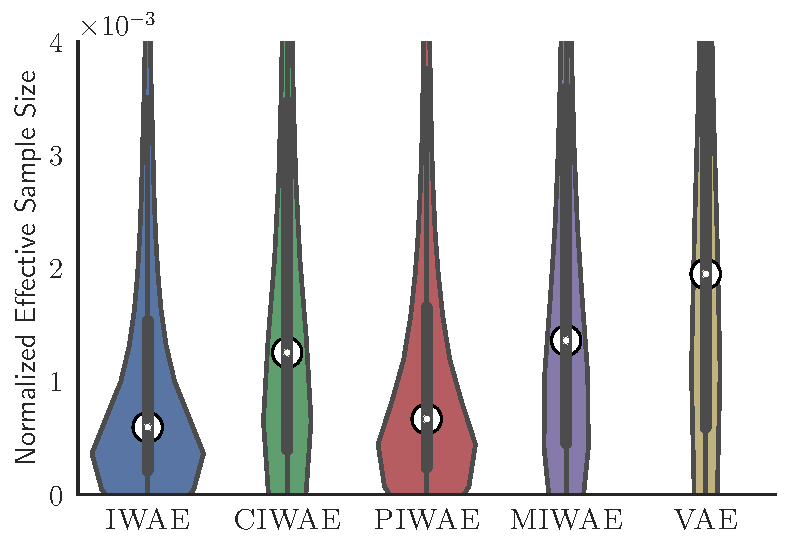
\includegraphics[width=0.39\textwidth]{figures/tighter_bounds/ess_violin}\vspace{-10pt}
	\caption{Violin plots of ESS estimates for each image of MNIST,
		normalized by the number of samples drawn. A violin plot uses a kernel density plot on each side -- thicker means more MNIST images whose $q_{\phi}$ achieves that ESS. 
		\vspace{-17pt}  \label{fig:violiness}}
\end{figure}

We next considered tuning the parameters for each of
our algorithms as shown in Figure~\ref{fig:mnistexpt/dotplot}, for
which we look at the final metric values after training.
Table~\ref{table:final-pef} further summarizes the performance
for certain selected parameter settings. For \gls{MIWAE} we see that as we increase $M$, 
the $\log \hat{p}(x)$ metric gets worse, while the \textsc{KL}
gets better.  The \gls{IWAE}-64  metric initially increases with $M$, before reducing
again from $M=16$ to $M=64$, suggesting that intermediate
values for $M$ (i.e. $M\neq1$, $K\neq1$) give a better trade-off.  For \gls{PIWAE}, similar
behavior to \gls{MIWAE} is seen for the \gls{IWAE}-64 
and \textsc{KL} metrics.  However, unlike for \gls{MIWAE}, we see that 
$\log \hat{p}(x)$ initially increases with $M$, such that 
\gls{PIWAE} provides uniform improvement over \gls{IWAE}
for the $M=2,4,8,$ and $16$ cases.  
\gls{CIWAE} exhibits similar behavior in increasing $\beta$
as increasing $M$ for \gls{MIWAE}, but there appears to
be a larger degree of noise in the evaluations, while the optimal
value of $\beta$, though non-zero, seems to be closer
to \gls{IWAE} than for the other algorithms.

As an additional measure of the performance of the inference
network that is distinct to any of the training targets, 
we also considered the effective sample size (ESS)~\cite{Mcbook}
for the fully trained networks, defined as
\begin{align}
\text{ESS} = (\textstyle \sum_{k=1}^K w_k)^2 / \textstyle \sum_{k=1}^K w_k^2.
\end{align}
The ESS is a measure of how many unweighted samples would be equivalent
to the weighted sample set.  
A low $\text{ESS}$ indicates that the inference network is struggling to
perform effective inference for the generative network.
The results, given in Figure~\ref{fig:violiness}, show that the
ESSs for \gls{CIWAE}, \gls{MIWAE}, and the \gls{VAE} were
all significantly larger than for \gls{IWAE} and \gls{PIWAE},
with \gls{IWAE} giving a particularly poor ESS.

Our final experiment looks at the \gls{SNR} values for the 
inference networks during training.  Here we took a number of different neural network gradient weights
at different layers of the network and calculated empirical estimates
for their \gls{SNR}s at various points during the training.  We then
averaged these estimates over the different network weights, the 
results of which are given in Figure~\ref{fig:inferencesnr}.  This
clearly shows the low \gls{SNR} exhibited by the \gls{IWAE}
inference network, suggesting that our results from the simple
Gaussian experiments carry over to the more complex neural network
domain.

 


\begin{figure}[t!]
	\centering
	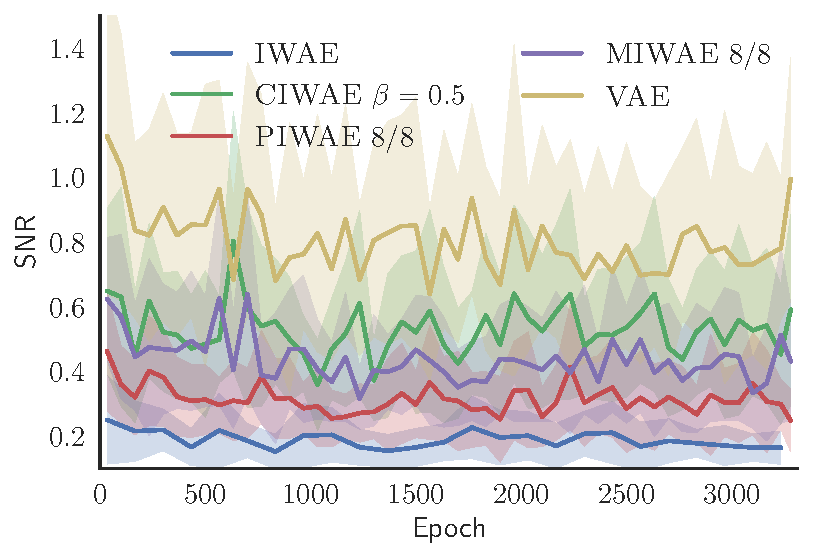
\includegraphics[width=0.395\textwidth]{figures/tighter_bounds/snr_encoder}
	\caption{\gls{SNR} of inference network weights during training. All lines are mean $\pm$ standard deviation over 20 randomly chosen weights per layer.
		\vspace{-12pt} \label{fig:inferencesnr}}
\end{figure}

